\documentclass[a4paper]{article}
\setlength{\headheight}{1.1\baselineskip}
\usepackage[english]{babel}
\usepackage[utf8x]{inputenc}
% package for including graphics with figure-environment
\usepackage{graphics}
\usepackage{hyperref}
% colors for hyperlinks
% colored borders (false) colored text (true)
\hypersetup{colorlinks=true,citecolor=black,filecolor=black,linkcolor=black,urlcolor=black}

% package for bibliography
\usepackage[authoryear,round]{natbib}
% package for expectation signs
\usepackage{amsmath,amssymb,mathtools,bm,etoolbox}
%\documentclass[a4paper,11pt]{report} 
\usepackage{breqn}
\usepackage{amsmath}
\usepackage{enumitem} 
\usepackage{amsmath, amsthm, amssymb}
\usepackage{amsmath}
\newcommand{\abs}[1]{ \left\lvert#1\right\rvert} 
\newcommand{\norm}[1]{\left\lVert#1\right\rVert}

% some more packages enabling table and figure production
\usepackage{float, afterpage, rotating, graphicx}
\usepackage{epstopdf}
\usepackage{longtable, booktabs, tabularx}
\usepackage{fancyvrb, moreverb, relsize}
\usepackage{eurosym, calc, chngcntr}
\usepackage{amsmath, amssymb, amsfonts, amsthm, bm}
\usepackage{caption}
\usepackage{mdwlist}
\usepackage{xfrac}
\usepackage{setspace}
\usepackage{xcolor}
\usepackage{multirow}
%\usepackage{booktabs}

\begin{document}
\section{Appendix}

\subsection{Empirical Definition of Trimming Function}
This paper comes up with an empirical way to employ trimming functions both for Ichimura's and Klein and Spady's methods.

Referring to theoretical definitions, the aim of a trimming function is to guarantee $\hat{p}_{-i}(X_i'\beta) = \frac{1}{nh}\sum_{j=1,j \neq i}^{n}K(\frac{X_j'\beta - X_i'\beta}{h})$ not too close to zero. Theoretically bounds $A_\delta$ and $A_n$ are imposed on exogenous variables.

To interpret, the estimate $\hat{p}_{-i}(X_i'\beta)$ is calculated over bandwidth $h$. There are two ways to keep such an estimate away from zero: either there exists enough many realizations of $X_i'\beta$ itself, corresponding to a theoretically high $p(x'\beta)$ guaranteed by $A_\delta$, or it is a point very close to $X_i'\beta$ (or $X_i$, since a linear transformation should not deviate the point much), which is denoted as $A_n$. The latter also leads to $\hat{p}_{-i}(X_i'\beta)$, the estimated probability for $X_i'\beta$ to be large enough. Furthermore, to avoid choosing inappropriate estimate for $\beta$, $A_n$ is implemented to calculate the leave-one-out NW estimator for g.

Following this interpretation, simulated sample data is sieved by examining whether their (more specifically, the single indices constructed on sample data) leave-one-out kernel estimates are large enough. If $\hat{p}(x'\beta)$ fails to achieve the chosen lower bound, this sample data $x$ will be removed from sample data set before turning to estimation step.

Furthermore, as we choose Grid Search method to carry out the estimation, the same set of grids is used to define $\mathcal{B}$, the support of $\beta$. And data sieving is carried out over this set such that the estimation procedure is sensible for each single grid.

To keep the comparability, the same set of trimmed data is used for both Ichimura's and Klein and Spady's estimation methods. However, this is not enough for the latter to work. While the initiative is to avoid any estimate of $g$ being too close to 0 or 1, a technically too small estimate may still emerge. The reason resides in coexistence of a large enough denominator and yet a relatively too small nominator (a number smaller than double epsilon is treated as zero in R language). Recollect that the nominator follows the sum of the binary variable $y_i$ weighted by its corresponding kernel evaluation, problem pops up when a relatively large evaluation coincides with $y_i = 0$. Therefore, based on the same trimmed data as in Ichimura's method, we further introduced a lower bound equals to square root of machine double epsilon and set any estimate smaller than the lower bound to this level.


\subsection{A Comparison in Results of Simulation Functions and NP Package}
Model design of monte carlo simulation following Ichimura (1993):
\begin{itemize}
\item sample size is 250;
\item the semiparametric single index model is specified as binary choice model;
\item exogenous vector of variables contains two components and both are independently generated from standard normal distribution;
\item when constructing single index, parameter of the first exogenous component is normalized to 1, and true value for the second parameter is set to -2;
\item presume standard normal distribution for error distribution;
\item the amount of monte carlo simulation is 1000 times.
\end{itemize}
To summarize, the designed baseline function is
\begin{equation*}
y_i = I(x_{1i} - 2x_{2i} > \epsilon_i).
\end{equation*}

\begin{table}[H]
\caption {Mean Squared Error Comparison} \label{tab:mean squared error}

(with gridsearch $(-4, 0, 81)$)

\begin{tabular}{l r r}

\toprule
\textbf{method} & \textbf{NP Package} & \textbf{Simulation Functions} \tabularnewline\midrule
(standard normal distribution for $x_1$, $x_2$, $\epsilon$) & &
\tabularnewline
Ichimura & 0.00363 & 0.00201 \tabularnewline
Klein and Spady & 0.00416 & 0.0000893 \tabularnewline

\bottomrule
\end{tabular}
\end{table}

\begin{figure}[h!]
  \caption{Comparison of Estimates on the Same Scale}
  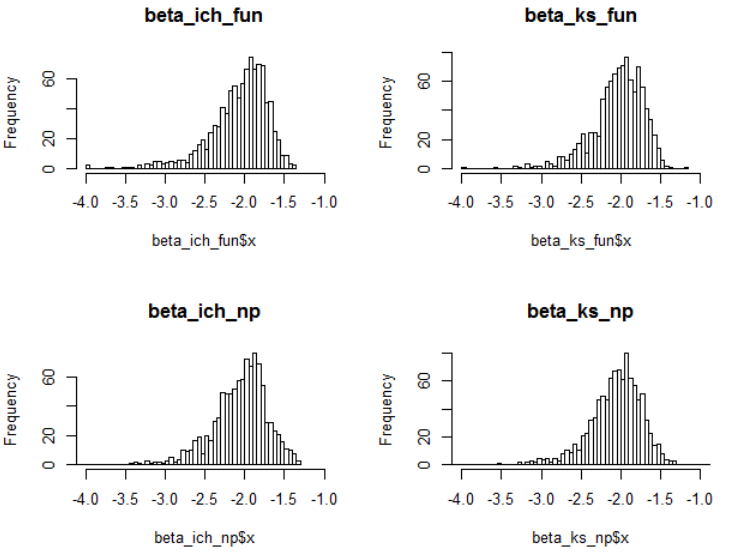
\includegraphics[width=\linewidth]{compare_done.png}
 
  \label{fig:comparison of estimates on the same scale}
\end{figure}

From $Table\ 3$ and $Figure\ 3$, we see that our self-implemented code does not perform significantly worse than the np package. In fact it is even better in the case with klein and spady function. This could be due to the use of our a priori knowledge of the true beta in specifying our grid. We thus conclude that it is an useful and successful practice in constructing our own code for single index model functions.

Nevertheless we take a further look into np package. It employs a nonlinear parameter estimation tool ($optim: Nelder-Mead$) which does not requires derivatives of objective function and uses heuristics to search the domain of parameter. Compared to the support of $\mathcal{B}$ prespecified in Grid Search, the core function that facilitates our research is $npindexbw$, which declares successful convergence in three ways: reaching absolute convergence tolerance, relative convergence tolerance or maximum number of iterations ($500$ times for Nelder-Mead method). Besides, this function provides a choice of different (random) initial points to start the searching, whereas in our simulation functions, starting points are manually chosen which may lead to ignorance of other local minima.

\subsection{Evidence for Decreasing Bias with Increasing Sample Size}
\begin{table}[H]
\caption {Bias Change for Various Sample Sizes} \label{tab:bias change}

$x_1$ and $x_2$ normal; a Monte Carlo experiment(1000 trials).
\centering
\resizebox{.75\textwidth}{!}{

\begin{tabular}{l r r r}
\toprule

Estimator  & n=50 & n=150 & n=250
\tabularnewline
\midrule
Ichi  & -0.1477 & -0.06515 & -0.04485
\tabularnewline
KS & 0.0299 & -0.03015 & -0.00945
\tabularnewline 
Logit  & -0.240235  & -0.05246 & -0.030321
\tabularnewline
\bottomrule
\end{tabular}
}
\end{table}
\end{document}